\documentclass[../main.tex]{subfiles}
\begin{document}
	
	\chapter{Álgebra Vetorial e Geometria Analítica}
	Para iniciar os estudos de Álgebra Linear, é interessante apresentar, inicialmente, conceitos básicos para visualizar e estruturar o conhecimento. Nesse sentido, entender vetores na perspectiva geométrica, ou seja, no plano ($\mathbb{R}^2$) ou no espaço ($\mathbb{R}^3$), é mais intuitivo em um primeiro contato. Nos próximos capítulos, em especial no capítulo 3, a definição de vetores será ampliada para outros espaços vetoriais, com um maior nível de abstração.
	
	\section{Álgebra Vetorial}
		\begin{definicao}
			\azul{Vetores (geometricamente)} são objetos matemáticos que possuem módulo, direção e sentido.
			
			Usualmente, um vetor é representado por segmentos de retas orientados equipolentes, ou seja, que apresentam mesmo tamanho, direção e sentido.
			\begin{center}
				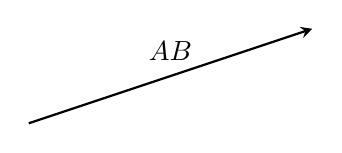
\begin{tikzpicture}[scale=1.2, >=stealth]
					\draw[thick] [->] (0,0) -- (3,1) node[midway, above=2pt] {$\vv{AB}$};
				\end{tikzpicture}
			\end{center}
		\end{definicao}
		Note que, pela definição, um vetor não possui "origem fixa" e pode ser representado por diferentes segmentos de reta orientados.
		\begin{definicao}
			Sejam $U$ e $V$ vetores representados por $\vv{AB}$ e $\vv{BC}$, respectivamente. A \azul{soma de vetores} $U+V$ é definida como o vetor representado pelo segmento de reta orientado $\vv{AC}$  
			\begin{center}
				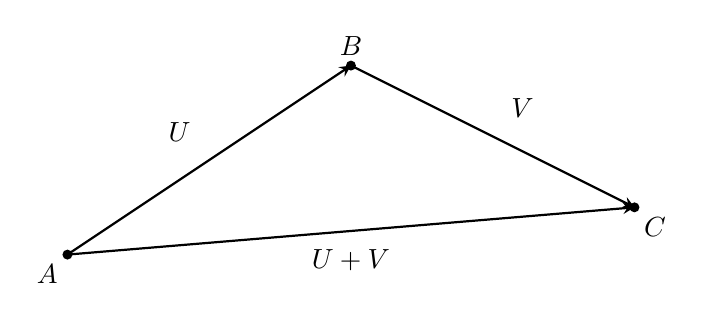
\begin{tikzpicture}[scale=1.2, >=stealth]
					% Pontos
					\coordinate (A) at (0,0);
					\coordinate (B) at (3,2);
					\coordinate (C) at (6,0.5);
					
					% Lados com setas
					\draw[thick, ->] (A) -- (B) node[midway, above left=3pt] {$U$};
					\draw[thick, ->] (B) -- (C) node[midway, above right=3pt] {$V$};
					\draw[thick, ->] (A) -- (C) node[midway, below=3pt] {$U+V$};
					
					% Pontos marcados
					\fill (A) circle (1.5pt) node[below left] {$A$};
					\fill (B) circle (1.5pt) node[above] {$B$};
					\fill (C) circle (1.5pt) node[below right] {$C$};
				\end{tikzpicture}
			\end{center}
		\end{definicao}
		\begin{proposicao}
			Sejam $V$, $W$ e $U$ vetores.
			A soma de vetores segue as seguintes propriedades:
			\begin{enumerate}[label=\roman*)]
				\item $V+W=W+V$ (comutatividade)
				\item $V+(W+U)=(V+W)+U$ (associatividade)
				\item $\exists \text{ vetor }\bar{0}\text{, tal que }  V+\bar{0}=V$ (existência do elemento neutro/vetor nulo)
			\end{enumerate}
		\end{proposicao}
		Abaixo seguem ilustrações das propriedades i) e ii).
		\begin{figure}[h!]
			\centering
			\begin{minipage}{0.45\textwidth}
				\centering
				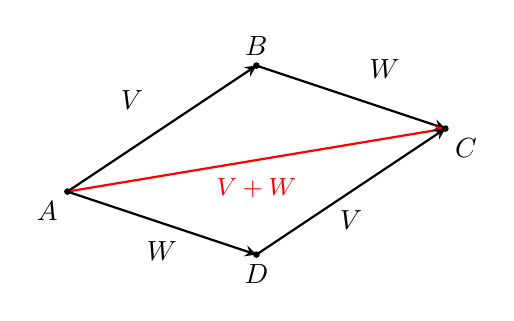
\begin{tikzpicture}[scale=0.8, >=stealth]
					% Pontos
					\coordinate (A) at (0,0);
					\coordinate (B) at (3,2);
					\coordinate (C) at (6,1);
					\coordinate (D) at (3,-1);
					
					% Lados com setas
					\draw[thick, ->] (A) -- (B) node[midway, above left=3pt] {$V$};
					\draw[thick, ->] (B) -- (C) node[midway, above right=3pt] {$W$};
					\draw[thick, ->, red] (A) -- (C) node[midway, below=3pt] {\small $V+W$};
					\draw[thick, ->] (A) -- (D) node[midway, below=3pt] {$W$};
					\draw[thick, ->] (D) -- (C) node[midway, below=3pt] {$V$};
					
					% Pontos marcados
					\fill (A) circle (1.5pt) node[below left] {$A$};
					\fill (B) circle (1.5pt) node[above] {$B$};
					\fill (C) circle (1.5pt) node[below right] {$C$};
					\fill (D) circle (1.5pt) node[below] {$D$};
				\end{tikzpicture}
			\end{minipage}
			\hfill
			\begin{minipage}{0.45\textwidth}
				\centering
				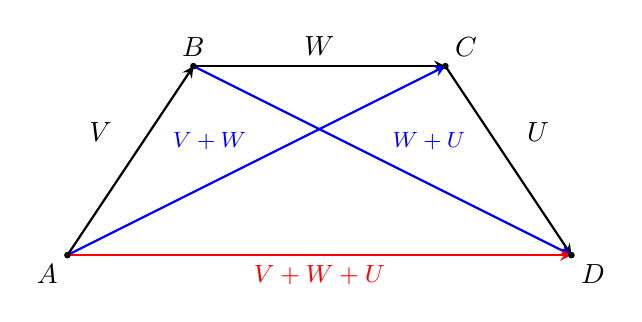
\begin{tikzpicture}[scale=0.8, >=stealth]
					% Pontos
					\coordinate (A) at (0,0);
					\coordinate (B) at (2,3);
					\coordinate (C) at (6,3);
					\coordinate (D) at (8,0);
					
					% Lados com setas
					\draw[thick, ->] (A) -- (B) node[midway, above left=3pt] {$V$};
					\draw[thick, ->] (B) -- (C) node[midway, above] {$W$};
					\draw[thick, ->] (C) -- (D) node[midway, above right=3pt] {$U$};
					\draw[thick, ->, blue] (A) -- (C) node[midway, above left] {\footnotesize $V+W$};
					\draw[thick, ->, blue] (B) -- (D) node[midway, above right] {\footnotesize $W+U$};
					\draw[thick, ->, red] (A) -- (D) node[midway, below] {\small $V+W+U$};
					
					% Pontos marcados
					\fill (A) circle (1.5pt) node[below left] {$A$};
					\fill (B) circle (1.5pt) node[above] {$B$};
					\fill (C) circle (1.5pt) node[above right] {$C$};
					\fill (D) circle (1.5pt) node[below right] {$D$};
				\end{tikzpicture}
			\end{minipage}
		\end{figure}
		\begin{definicao}
			Seja $V$ um vetor. Seu \azul{simétrico}, denotado por $-V$, é o vetor tal que
			\[
			V+(-V)=\bar{0}
			\]
		\end{definicao}
		\begin{definicao}
			Sejam $V$ e $W$ vetores. A \azul{diferença $W$ menos $V$} é definida como
			\[
			W-V=W+(-V)
			\]
		\end{definicao}
		\begin{definicao}
			Sejam $V\neq \bar{0}$ um vetor e $\alpha\neq 0$ um escalar (ou seja, um número real). A \azul{multiplicação do vetor $V$ por um escalar $\alpha$}, denotada por $\alpha V$, é definida pelo vetor tal que:
			\begin{enumerate}[label=\roman*)]
				\item seu módulo é $|\alpha|\cdot |V|$, onde $|V|$ é o módulo de $V$;
				\item a direção é a mesma de $V$;
				\item tem sentido de $V$ se $\alpha>0$, e sentido de $-V$ se $\alpha<0$.
			\end{enumerate}
			Caso $V=\bar{0}$ ou $\alpha=0$, $\alpha V=\bar{0}$
		\end{definicao}
		\begin{definicao}
			Seja $V$ um vetor. As \azul{componentes de V} são cada elemento das coordenadas que representam o ponto final com relação à origem do sistema de coordenadas escolhido.
			
			Se $V$ está no plano (\azul{$\mathbb{R}^2$} ou \azul{espaço euclidiano bidimensional}), então suas coordenadas são uma trupla de dois números reais, denotadas usualmente por $(v_1, v_2)$.
			
			Se $V$ está no espaço (\azul{$\mathbb{R}^3$} ou \azul{espaço euclidiano tridimensional}), então suas coordenadas são uma tupla de três números reais, denotadas usualmente por $(v_1, v_2, v_3)$.
			
			Se $V$ está em "dimensões maiores" (\azul{$\mathbb{R}^n$} ou \azul{espaço euclidiano n-dimensional}), então suas coordenadas são uma tupla de $n$ números reais, denotadas usualmente por $(v_1, \dots, v_n)$.
		\end{definicao}
		Abaixo seguem ilustrações de como coordenadas funcionam no plano e no espaço.
		\begin{figure}[h]
			\centering
			
			% --- subfigura R^2 ---
			\begin{subfigure}[t]{0.48\textwidth}
				\centering
				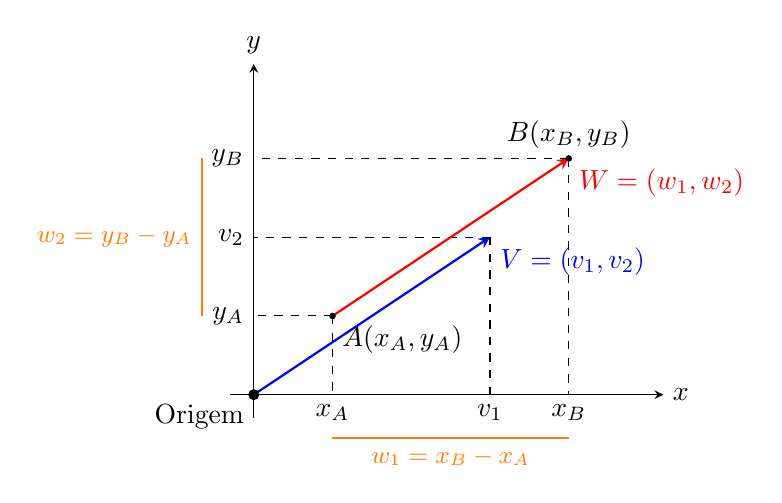
\begin{tikzpicture}[>=stealth,scale=1.0] % pode ajustar a escala se quiser
					% Eixos
					\draw[->] (-0.3,0) -- (5.2,0) node[right] {$x$};
					\draw[->] (0,-0.3) -- (0,4.2) node[above] {$y$};
					
					\coordinate (O) at (0,0);
					\coordinate (P) at (3,2);   % ponto de v
					\coordinate (A) at (1,1);   % ponto inicial de w
					\coordinate (B) at (4,3);   % ponto final de w
					
					% Vetor na origem
					\draw[->,thick,blue] (O) -- (P)
					node[below right] {$V=(v_1,v_2)$};
					
					% Projeções de v
					\draw[dashed] (P) -- (3,0) node[below] {$v_1$};
					\draw[dashed] (P) -- (0,2) node[left] {$v_2$};
					
					% Vetor deslocado
					\draw[->,thick,red] (A) -- (B)
					node[below right] {$W=(w_1,w_2)$};
					
					% Pontos A e B e orgigem
					\fill (A) circle (1.2pt) node[below right] {$A(x_A,y_A)$};
					\fill (B) circle (1.2pt) node[above] {$B(x_B,y_B)$};
					\fill (O) circle (2pt) node[below left] {\text{Origem}};
					
					% Projeções para mostrar diferenças
					\draw[dashed] (A) -- (1,0) node[below] {$x_A$};
					\draw[dashed] (B) -- (4,0) node[below] {$x_B$};
					\draw[dashed] (A) -- (0,1) node[left] {$y_A$};
					\draw[dashed] (B) -- (0,3) node[left] {$y_B$};
					
					% Segmentos representando as diferenças
					\draw[thick,orange,yshift=-10pt]
					(1,-0.2) -- node[below] {\small $w_1 = x_B - x_A$} (4,-0.2);
					
					\draw[thick,orange,xshift=-13pt]
					(-0.2,1) -- node[left] {\small $w_2 = y_B - y_A$} (-0.2,3);
				\end{tikzpicture}
				\caption{Representação no $\mathbb{R}^2$.}
			\end{subfigure}
			\hfill
			% --- subfigura R^3 ---
			\begin{subfigure}[t]{0.48\textwidth}
				\centering
				\tdplotsetmaincoords{70}{120}
				\begin{tikzpicture}[scale=1.6,tdplot_main_coords,>=stealth]
					% Eixos
					\draw[->] (0,0,0) -- (3,0,0) node[below right] {$x$};
					\draw[->] (0,0,0) -- (0,3,0) node[left] {$y$};
					\draw[->] (0,0,0) -- (0,0,3) node[above] {$z$};
					
					% Vetor na origem
					\coordinate (V) at (1,1.4,3);
					\draw[->,thick,blue] (0,0,0) -- (V)
					node[below right] {$V=(v_1,v_2,v_3)$};
					\fill (0,0,0) circle (1.5pt) node[above left] {\text{Origem}};
					\fill (V) circle (1.5pt) node[above left] {};
					
					% Projeções de v
					\coordinate (Vxy) at (1,1.4,0);
					\coordinate (Vx)  at (1,0,0);
					\coordinate (Vy)  at (0,1.4,0);
					\draw[dashed] (V) -- (Vxy);
					\draw[dashed] (Vxy) -- (Vx) node[above left] {$v_1$};
					\draw[dashed] (Vxy) -- (Vy) node[above right] {$v_2$};
					\draw[dashed] (V) -- (0,0,3) node[left] {$v_3$};
					\draw[dashed] (0,0,0) -- (Vxy);
				\end{tikzpicture}
				\caption{Representação no $\mathbb{R}^3$.}
			\end{subfigure}
			
			\caption{Componentes de vetores em $\mathbb{R}^2$ e $\mathbb{R}^3$.}
			\label{fig:vetores-R2-R3}
		\end{figure}
		
		Perceba que, para verificar as componentes de um vetor qualquer $W$ representado por um segmento $\vv{AB}$, basta subtrair as suas coordenadas, de modo que:
		\[
		W = \vv{AB}\Rightarrow
		\begin{cases}
			w_1 = x_B - x_A\\
			w_2 = y_B - y_A
		\end{cases}\Rightarrow
		W = (x_B - x_A,\, y_B - y_A)
		\]
		Para o $\mathbb{R}^3$, a subtração ocorre da mesma forma.
		
		Com isso, note que as operações ficam muito mais fáceis, sem depender sempre do apelo geométrico. Assim, podemos buscar uma nova forma de fazer as operações básicas entre vetores (soma e multiplicação por escalar):
		\begin{proposicao}
			
		\end{proposicao}
	\section{Geometria Analítica}
	\section{Matrizes como Vetores}
	
\end{document}
